\documentclass[12pt]{report}
\usepackage{mathpartir}
\usepackage{amsmath}
\usepackage{amssymb}
\usepackage{multicol}
\usepackage[utf8x]{inputenc}
\usepackage[french]{babel}
\usepackage{graphicx}

\title{Typage d'un lambda-calcul avec une construction de branchements}
\author{Frédéric Bour, avec l'encadrement de Yann Régis-Gianas}

\newcommand\todo[1]{TODO[#1]}
\includeonly{langage}

\begin{document}

\maketitle

%%%%%%%%%%%%%%%%%%%%%%%%%%%%%%%%%%%%%%%%%%%%%%%%%%%%%%%%%%%%%%%%%%%%%%%%%%%%%%%%
%%%%%%%%%%%%%%%%%%%%%%%%%%%%%%%%%%%%%%%%%%%%%%%%%%%%%%%%%%%%%%%%%%%%%%%%%%%%%%%%

\chapter{Motivations}

Ce TRE a débuté par une évaluation de la faisabilité d'une analyse statique du
flot des exceptions pour OCaml 4.00. 

Les systèmes d'exceptions permettent au programmeur de manipuler le contrôle de
flot beaucoup plus librement qu'avec un traditionnel appel de fonction
retournant une valeur. Malheureusement, il devient alors difficile de connaître
les différents flots d'exécutions possibles car ceux-ci ne correspondent plus
strictement à la structure du code source -- on parle de contrôle de flot
non-local.

Bien qu'OCaml soit reconnu pour la sûreté des programmes écrits avec, il faut
souvent se priver d'exceptions pour garantir celle-ci.

L'analyse statique que nous souhaitions effectuer vise à vérifier de manière
mécanique l'absence d'exceptions ou bien l'exhaustivité de leur traitement dans
un code source.

Ce travail reprenait les résultats de la thèse de François Pessaux \todo{ref
these} qui avait abouti à un prototype permettant ce type d'analyse pour OCaml
3.00.  Les résultats étaient très encourageants au point de présenter un
intérêt immédiat pour des applications industrielles (\todo{ref ocamlpro ?}).

Malheureusement, ce prototype n'a pas été porté vers les versions suivantes
d'OCaml et nous sommes arrivé à la conclusion que ce travail était trop
conséquent pour s'inscrire dans le cadre d'un TRE.  De plus, si l'approche
abordée dans la thèse permet une analyse fine, l'implantation est difficile à
maintenir car celle-ci s'appuie sur la syntaxe abstraite d'OCaml et implique de
développer en parallèle un typeur spécialisé.

Notre travail de recherche s'est alors orienté vers le langage intermédiaire du
compilateur OCaml. 

\section{\emph{Lambda}, le langage intermédiaire}

Cibler \emph{Lambda} apporte de nombreux avantages, notamment :
\begin{description}
  \item[Indépendance vis-à-vis du \emph{front-end}]. Si le langage de surface
    OCaml est régulièrement étendu, \emph{Lambda} est très stable et n'a pas
    connu de changements majeurs depuis l'introduction du système objet il y a
    plus de 10 ans. C'est une cible pérenne.(\todo{ref OO})
  \item[Langage minimaliste].
    Les nombreuses constructions de surface sont réduites à un petit ensemble.
    \todo{facteur 10 entre TypedTree et lambda}.
    L'analyse peut ainsi se concentrer directement sur le cœur du langage et
    garder une taille modeste. Le travail de maintenance est moindre.
\end{description}

Cependant, ce langage n'est pas typé. Dans la chaîne de traitement du
compilateur, les types sont vérifiées pour le langage source par le typeur puis
effacé. Tout le reste du traitement s'effectue sur une version non-typée du
programme sémantiquement équivalente. Ce choix est justifié compte par
l'omniprésence du polymorphisme paramétrique dans ce langage et de la
représentation très régulière des valeurs à l'exécution.

Le polymorphisme paramétrique offre la garantie qu'un programme bien typé est
équivalent après effacement des types \todo{ref didier rémy ?}, et la
représentation des valeurs permet au \emph{runtime} de travailler correctement
sans information de types -- cela concerne par exemple la convention d'appel
des fonctions ou le passage du glâneur de cellule.

\todo{figure : pipeline ocaml}.

Ce choix restreint les traitements possibles dans la suite de la compilation.
Le compilateur natif tente par exemple de réinférer des types dans le cadre de
certaines optimisations, mais il ne s'agit que d'approximation conservative.
Dans notre cas analyser le flot devient beaucoup plus compliqué -- un travail
absurde quand on sait que les informations nécessaires pour guider correctement
cette analyse viennent d'être effacées dans la chaîne de compilation.

Avant d'avoir un outil d'analyse respectant cette architecture, il fallait donc
concevoir une version de \emph{lambda} préservant les types.

\section{Vers une version \emph{typée} de \emph{Lambda}}

Le langage \emph{lambda} est un lambda-calcul proposant des fonctions de très
bas-niveau.

Dans le cadre de la compilation, le lambda-calcul désigne une famille de
langage de programmation fonctionnelle reposant autour d'un unique mécanisme
d'abstraction.  Cela rend sa définition simplissime, le noyau syntaxique tient
en trois règles.  Mais derrière celles-ci se cache une très grande expressivité
: c'est un langage turing-complet et d'un suffisamment haut-niveau pour
permettre un encodage léger des constructions classiques des langages de
programmation.  (\todo{cite appel, steele, ?}).

Un lambda-calcul est ainsi un choix naturel pour un langage intermédiaire. La
variante d'OCaml ajoute principalement des primitives d'accès mémoires et de
branchements, des extensions de bas-niveau.

Une autre implantation majeure d'un langage de programmation fonctionnelle
proche de ML, \todo{ref GHC}, a fait un choix très différent dans la conception
de son langage intermédiaire nommé \emph{Core}.  Ce dernier est typé et n'offre
pas de telles primitives; les accès mémoires sont masqués derrière une forme
simplifiée de \emph{filtrage de motifs}.  \todo{cite System FC} Ce design
influencera nos choix par la suite.

\section{Le typage des constructions de bas-niveau}

Les systèmes de types d'Ocaml et d'Haskell présentent de nombreuses
similarités. La réussite de \emph{Core} nous a conforté dans la faisabilité
d'un traitement similaire pour OCaml.

Cependant dans le soucis d'être le moins intrusif possible dans le compilateur
OCaml actuel, il était nécessaire d'étendre le langage \emph{lambda} et non de
le remplacer.

Pour mener à terme cet objectif, les étapes suivantes se profilaient :
\begin{itemize}
  \item concevoir un système de type s'inspirant de System $F_c$ et composant
    avec les contraintes imposées par \emph{lambda},
  \item établir encodage des constructions d'Ocaml (types algébriques, modules,
    GADTs, variants polymorphes) dans ce système afin de s'assurer que toutes
    sont capturées,
  \item étendre \emph{lambda} et proposer un schéma de compilation vers ce
    nouveau langage intermédiaire.
\end{itemize}

Ceci constitue un travail de grande ampleur. Dans ce rapport nous adressons le
le point précis de typer les contraintes imposées par \emph{lambda}; un
branchement et des accès mémoires beaucoup plus libre que ce que ne permet le
\emph{filtrage de motif} traditionnel.



%%%%%%%%%%%%%%%%%%%%%%%%%%%%%%%%%%%%%%%%%%%%%%%%%%%%%%%%%%%%%%%%%%%%%%%%%%%%%%%%
%%%%%%%%%%%%%%%%%%%%%%%%%%%%%%%%%%%%%%%%%%%%%%%%%%%%%%%%%%%%%%%%%%%%%%%%%%%%%%%%

\chapter{Solutions étudiées}

Tout n'est pas nécessaire, points principaux :

\section{Échec du typage structurel}

\subsection{Succès du typage nominal}

- encodage des exceptions
- encodage des GADTs
- encodage des variants
  - traduction du langage ML
    shift, extraction de tags, …

%%%%%%%%%%%%%%%%%%%%%%%%%%%%%%%%%%%%%%%%%%%%%%%%%%%%%%%%%%%%%%%%%%%%%%%%%%%%%%%%
%%%%%%%%%%%%%%%%%%%%%%%%%%%%%%%%%%%%%%%%%%%%%%%%%%%%%%%%%%%%%%%%%%%%%%%%%%%%%%%%

\section{Conception d'un langage approprié}

Le langage développé reprend le cœur du lambda-calcul polymorphe
\cite{Reynolds94anintroduction} (aussi connu sous le nom de \emph{Système F})
et l'étend avec les notions de primitives et de \emph{bloc} muni d'un
\emph{tag} et les constructions d'analyse de tag et d'aiguillage.

Présentons tout d'abord le noyau de ce langage.

\subsection{Lambda-calcul polymorphe} 

Les trois premières constructions du langage sont les variables, l'application
et l'abstraction. Elles forment lambda-calcul simplement typé.

Ces trois constructions permettent de construire et d'appliquer des fonctions,
dont le type est noté par une \emph{flèche} paramétrée par le domaine et le
codomaine de la fonction.

L'application et l'abstraction de types rajoutent le polymorphisme, représenté
au niveau des types par la quantification universelle.

Contrairement à un langage tel qu'OCaml, la généralisation et l'instantiation
des valeurs polymorphes sont marquées explicitement. Si un tel langage devait
être utilisé dans le compilateur, c'est lors de la traduction que celles-ci
seraient ajoutées par le \emph{frontend}.

\subsection{Représentation des valeurs d'OCaml}

Les extensions ont été conçues autour de la représentation des valeurs par
OCaml. Les valeurs concrètes sont :
\begin{itemize}
  \item soit des entiers, directement représenté par un scalaire,
  \item soit des blocs représentés par un pointeur vers une
zone mémoire composée d'un \emph{tag} et d'un vecteur de valeurs.
\end{itemize}
Un bit des valeurs est réservé pour distinguer les entiers des pointeurs.

\begin{figure}
\centering
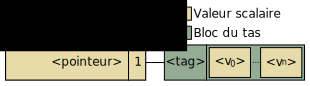
\includegraphics{media/ocaml_value}
\caption{Forme des valeurs}
\end{figure}

\paragraph{Types algébriques}

La spécificité de ML qui marque sans doute le plus ceux qui aprennent ce langage
sont les \emph{types sommes}. Les types de cette forme ont plusieurs
constructeurs de valeurs.

Ce comportement rappelle les \emph{union}s du C, mais les constructeurs des
types sommes sont disjoints : une fois construit, on peut retrouver sans
ambiguité le constructeur qui a engendré une valeur. Enfin, ces constructeurs
peuvent recevoir des paramètres. 

\begin{lstlisting}
  type address =
    | Any
    | Localhost
    | IP of int * int * int * int
    | Host of string

  let resolve addr = match addr with
    | Any -> 0, 0, 0, 0
    | Localhost -> 127, 0, 0, 1
    | IP (a,b,c,d) -> a, b, c ,d
    | Host host -> (* getaddrinfo ... *)
\end{lstlisting}

Ici, \emph{Any} est constant : il n'existe qu'une seule valeur de type
\emph{address} issue de ce constructeur. De même pour \emph{Localhost}, mais
cette unique valeur est différente de celle d'\emph{Any}. \emph{IP} et
\emph{Host} sont paramétrés.  L'analyse des constructeurs paramétrés constitue
un mécanisme sûr et vérifiable pour transporter des valeurs de différents types.

Les constructeurs constants sont encodés par des entiers, les constructeurs
paramétrés par un bloc de même arité.

La valeur des entiers et le tag des blocs servent à discriminer les différents
constructeurs durant le \emph{filtrage de motif}. Les entiers endossent ainsi
le même rôle que le \emph{tag} des blocs; ceux-ci sont testés dynamiquement
pour choisir un branchement.

L'encodage du type \emph{address} est le suivant :
\begin{description}
  \item[Any] l'entier 0
  \item[Localhost] l'entier 1
  \item[IP] un bloc de tag 0 et d'arité 4
  \item[Host] un bloc de tag 1 et d'arité 1
\end{description}

\paragraph{Variants polymorphes} 
Les variants polymorphes sont une forme plus souple de types sommes. En
particulier, ils ne nécessitent pas de déclarations préalables et peuvent
s'étendre. Dans l'analyse d'une de ces valeurs, cela se matérialise par la
présence de cas « par défaut ».

L'encodage ressemble à celui des types sommes, mais le \emph{tag} pour
discriminer les constructeurs paramétrés n'est plus celui du bloc. Une
indirection est ajoutée sous la forme d'un premier bloc composé du \emph{tag}
et d'un pointeur vers un n-uplet contenant les paramètres.

Du point de vue du langage intermédiaire, le \emph{tag} devient ici une valeur
de première classe, manipulable dans le langage.  En particulier, celui-ci
peut-être testé et transformé par l'application d'opérateurs.

\begin{figure}
\centering
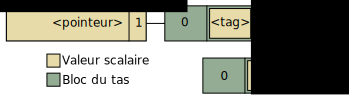
\includegraphics{media/ocaml_variant}
\caption{Forme des variants polymorphes}
\end{figure}

\subsection{Séparer extraction et analyse d'un \emph{tag}}

La principale contribution réside entre la séparation du calcul d'un tag et du
branchement qui s'ensuivra.

\paragraph{Filtrage de motif} Le \emph{filtrage de motif} est la construction
qui permet l'analyse des valeurs de types sommes pour sélectionner une branche
d'exécution.

Les différents constructeurs d'un type algébrique mènent chacun à une branche
différente. Dans chacune, des noms liés aux paramètres du constructeur
testé sont introduits. Le programmeur n'indique jamais explicitement l'accès
aux champs d'une valeur. Il ne peut même pas nommer un champ en dehors de la
branche.

Il est alors simple de vérifier l'exhaustivité du traitement et de garantir
l'absence d'accès à des valeurs inexistantes lors de l'exécution. Enfin le
compilateur se voit offrir beaucoup de libertés pour générer du code efficace,
différentes méthodes sont étudiées dans \cite{LeFessant:2001:OPM:507669.507641}
puis \cite{Maranget:2008:CPM:1411304.1411311}.

\paragraph{Motifs compilés} Le compilateur OCaml choisit de compiler ces motifs
très tôt. Dans le langage \emph{Lambda} il n'existe déjà plus que deux formes
de tests, les \emph{switch} et \emph{if} que l'on retrouve dans les langages
impératifs classiques. Une forme spécialisée de branchement proche du
\emph{goto} est aussi proposée pour factoriser le code des branches.

Les filtrages de haut-niveau sont ainsi traduits via des arbres de décisions,
au travers d'une suite de tests et de tables de sauts.  Le lien entre la
sélection d'une branche et les hypothèses qui y ont amené disparaît -- le
compilateur ne peut que suivre les instructions de projection sous l'hypothèse
que le code traduit est correct.

Voici le corps de la forme compilée de la fonction \emph{resolve} définie
ci-dessus :

\lstset{language=Lisp}
\begin{lstlisting}
(switch* addr
   ;; Any
   case int 0: [0: 0 0 0 0]
   ;; Localhost
   case int 1: [0: 127 0 0 1]
   ;; IP
   case tag 0:
    (makeblock 0 (field 0 addr) (field 1 addr)
      (field 2 addr) (field 3 addr))
   ;; Host
   case tag 1: ...)
\end{lstlisting}
\lstset{language=Caml}

Le lien entre une branche et la sélection qui y a mené est devenu implicite.
En particulier les projections dans la branche "IP", matérialisée par la
primitive \emph{field}, sont impossibles à vérifier.

Notre travail sur \emph{Lambda} vise à justifier la compilation de ces motifs ;
pour cela il faudra être capable de corréler statiquement la valeur d'un tag et
le type de la valeur \emph{taguée}.


%%%%%%%%%%%%%%%%%%%%%%%%%%%%%%%%%%%%%%%%%%%%%%%%%%%%%%%%%%%%%%%%%%%%%%%%%%%%%%%%
%%%%%%%%%%%%%%%%%%%%%%%%%%%%%%%%%%%%%%%%%%%%%%%%%%%%%%%%%%%%%%%%%%%%%%%%%%%%%%%%

% Metavars
\newcommand\term{t}
\newcommand\ty{\tau}
\newcommand\tyenv{\Gamma}
\newcommand\csenv{C}

% Term
\newcommand\var{x}
\newcommand\app[2]{#1\,#2}
\newcommand\lam[2]{\lambda #1. #2}

% Value
\newcommand\val{v}

% Type
\newcommand\tyconst{\iota}
\newcommand\tyvar{\alpha}
\newcommand\tykind{*}
\newcommand\tyarrow[2]{#1 \rightarrow #2}

% Binding
\newcommand\binding[2]{(#1 : #2)}

% Typing environment
\newcommand\tyenvnil{\bullet}
\newcommand\tyenvcons[3]{#1; \binding{#2}{#3}}

% Jugements
\newcommand\tycheck[3]{#1 \vdash #2 : #3}
\newcommand\tyenvmem[2]{#1 \in #2}

% Keyword
\newcommand\kw[1]{\operatorname{#1}}

% Syntax
\newcommand\syn[1]{#1 ::=& \; }
\newcommand\synor{\\ |& \; }
\newcommand\syndesc[1]{& \text{#1}}

% Pattern
\newcommand\pator{\;|\;}

% Operation semantic
\newcommand\redto[2]{#1 \longrightarrow #2}

\chapter{Langage proposé}

\section{Syntaxe}

\begin{figure}
\begin{align*}
  \syn{\term_1, \term_2} \var, y 
    \syndesc{variable}
  \synor      \term_1 \, \term_2
    \syndesc{application}
  \synor      \lambda \binding{\var}{\ty} . \term
    \syndesc{abstraction}
  \synor      \Lambda \tyvar . \term
    \syndesc{abstraction de type}
  \synor      \term \, \ty
    \syndesc{application de type}
  \synor      prim \, \vec{\term}
    \syndesc{application de primitives}
%  \synor      \kw{letrec} \vec{\var_i : \ty_i = \term_i} \kw{in} \term
  \synor      \kw{switch} \term \kw{in} \vec{b} : \ty
    \syndesc{aiguillage}
  \synor      \kw{unpack} \term_1 \kw{as} \var \kw{in} \term_2
    \syndesc{ouverture d'un bloc}
\end{align*}
\caption{Syntaxe des termes}
\end{figure}

\begin{figure}
\begin{align*}
  \syn{b} n \rightarrow \term \; | \; b
    \syndesc{cas constant}
  \synor  \_ \rightarrow \term
    \syndesc{cas par défaut}
  \synor  \emptyset
    \syndesc{absence de cas par défaut}
\end{align*}
\caption{Clauses de branchement}
\end{figure}

\begin{figure}
\begin{align*}
  \syn{\ty_1, \ty_2} \tyvar, \beta
    \syndesc{variables de type}
  \synor  \ty_1 \rightarrow \ty_2
    \syndesc{type flèche}
  \synor  \forall \tyvar. \ty
    \syndesc{quantification universelle}
  \synor  D
    \syndesc{type construit}
  \synor  \{ \var \}_D
    \syndesc{type \emph{singleton}}
  \synor  \kw{Tag}_z \var
    \syndesc{type du \emph{tag} d'un \emph{singleton}}
  \synor  \{ n: \vec{\ty} \}
    \syndesc{type d'un bloc immédiat}
  \\
  \syn{D} \epsilon \, \vec{\ty}
    \syndesc{constructeur paramétré}
\end{align*}
\caption{Syntaxe des types}
\end{figure}

\begin{figure}
\begin{align*}
  \syn{C} C \wedge C
    \syndesc{conjonction}
  \synor  \ty_1 = \ty_2
    \syndesc{égalité de types}
  \synor  \kw{tag} \var \in S
    \syndesc{restriction d'un \emph{tag}}
  \synor  \top
    \syndesc{Vrai}
  \synor  \bot
    \syndesc{Faux}
\end{align*}
\caption{Syntaxe des contraintes}
\end{figure}

\begin{figure}
\begin{align*}
  \syn{S} \emptyset
    \syndesc{ensemble vide}
  \synor  \{ k_1, \ldots, k_n \}
    \syndesc{ensemble fini}
  \synor  \lnot \{ k_1, \ldots, k_n \}
    \syndesc{complémentaire}
\end{align*}
\caption{Ensemble de \emph{tags}}
\end{figure}

\begin{figure}
\begin{align*}
  \syn{\tyenv} .
    \syndesc{contexte vide}
  \synor \tyenv \binding{\var}{\ty}
    \syndesc{liaison de terme}
  \synor \tyenv \binding{\alpha}{*}
    \syndesc{liaison de type}
\end{align*}
\caption{Syntaxe des contextes}
\end{figure}

\begin{figure}
\begin{align*}
  \syn{prim} \kw{makeblock}_{n,D}
    \syndesc{allocation d'un bloc}
  \synor \kw{tagof}
    \syndesc{extraction d'un \emph{tag}}
  \synor \kw{field}_{n}
    \syndesc{projection d'un champ}
  \synor \kw{eq}_{z}
    \syndesc{égalité}
  \synor \kw{lt}_{z}
    \syndesc{infériorité}
  \synor \kw{isint}
    \syndesc{test d'entier}
  \synor \kw{isout}_{[z1,z2]}
    \syndesc{test d'intervalle}
  \synor \kw{shift}_{z}
    \syndesc{décalage constant}
\end{align*}
\caption{Primitives du langage}
\end{figure}

\pagebreak

\section{Règles de typage}

\begin{mathpar}

\infer{
  \tyenvmem{\binding\var\ty}\tyenv
}{
  \tycheck\tyenv\var\ty
}

\infer{
  \tycheck{\csenv, \tyenvcons\tyenv\var{\ty_1}}{\term}{\ty_2}
}{
  \tycheck{\csenv, \tyenv}{\lam{\binding\var{\ty_1}}{\term}}{\tyarrow{\ty_1}{\ty_2}}
}

\infer{
  \tycheck{\csenv, \tyenv}{\term_1}{\tyarrow{\ty_1}{\ty_2}} \\
  \tycheck{\csenv, \tyenv}{\term_2}{\ty_1}
}{
  \tycheck{\csenv, \tyenv}{\term_1 \term_2}{\ty_2}
}

%\infer{
%  \forall i.\; \tycheck{\csenv, \tyenvcons{\tyenv}{\forall j.\, \var_j}{\ty_j}}{\term_i}{\ty_i} \\
%  \tycheck{\csenv, \tyenvcons{\tyenv}{\forall j.\, \var_j}{\ty_j}}{\term}{\ty}
%}{
%  \tycheck{\csenv, \tyenv}{\kw{letrec} (\var_i : \ty_i = \term_i) \kw{in} \term}{\ty}
%}

\\

\infer{
  \tycheck{\csenv, \tyenvcons{\tyenv}{\tyvar}{\tykind}}{\term}{\ty}
}{
  \tycheck{\csenv, \tyenv}{\Lambda \tyvar . \term }{\forall \tyvar.\, \ty}
}

\infer{
  \tycheck{\csenv, \tyenv}{\term}{\forall \tyvar.\, \ty_1}
}{
  \tycheck{\csenv, \tyenv}{\term \, \ty_2}{\ty_1 \{\tyvar \leftarrow \ty_2\}}
}

\\

\infer{
  x \notin \kw{dom}(\tyenv) \\ x \notin \kw{FV}(\ty) \\
  \tycheck{\csenv, \tyenv}{\term_1}{D} \\
  \tycheck{\csenv, \tyenvcons{\tyenv}
                             {\var}{ \{ \var \}_D }}
          {\term_2}{\ty}
}{
  \tycheck{\csenv, \tyenv}{\kw{unpack} \term_1 \kw{as} \var \kw{in} \term_2}{\ty} \\
}

\\

\infer{
  k \in dom(D) \\
  \tycheck{\csenv \wedge \kw{tag} \var \in \{ k \} \wedge D k, \tyenv}{\term}{\ty} \\
  \tycheck{\csenv \wedge \kw{tag} \var \in \lnot \{ k \}, x, D, \tyenv}{\vec{b}}{\ty}
}{
  \tycheck{\csenv, \tyenv, x, D}{k \rightarrow \term \;|\; \vec{b}}{\ty}
}

\infer{
  \tycheck{\csenv, \tyenv}{\term}{\ty}
}{
  \tycheck{\csenv, \tyenv, x, D}{\_ \rightarrow \term}{\ty}
}

\infer{
  %FIXME: from constraints, we deduce tag = empty%
  \csenv \Vdash dom(D) \cap \kw{tag} x = \emptyset
}{
  \tycheck{\csenv, \tyenv, x, D}{\emptyset}{\ty}
}

\infer{
  \tycheck{\csenv, \tyenv}{\term}{\{ \var \}_D} \\
  \tycheck{\csenv, \tyenv, \var, D}{\vec{b}}{\ty}
}{
  \tycheck{\csenv, \tyenv}{\kw{switch} \term \kw{in} \vec{b}}{\ty}
}

\end{mathpar}

\section{Type des primitives}
\begin{mathpar}

\infer{
  \tycheck{\csenv, \tyenv}{\term}{\{ \var \}_D}
}{
  \tycheck{\csenv, \tyenv}{\kw{tagof} \term}{\kw{Tag} \{ \var \}_D}
}


\infer{
  \tycheck{\csenv, \tyenv}{\term}{\{ k: \vec{\ty_n} \}}
}{
  \tycheck{\csenv, \tyenv}{\kw{field}_i \term}{\ty_i}
}

\infer{
  \tycheck{\csenv, \tyenv}{\term}{\{ k: \vec{\ty_n} \}}
}{
  \tycheck{\csenv, \tyenv}{\kw{field}_i \term}{\ty_i}
}

\infer{
  k \in dom(D) \\
  \tycheck{\forall i. \, \csenv, \tyenv}{\term_i}{D_{k,i}} \\
}{
  \tycheck{\csenv, \tyenv}{\kw{makeblock}_{k,D} \vec{\term_n}}{D}
}

\infer{
  \tycheck{\csenv, \tyenv}{\term}{\kw{Tag}_z \var} \\
}{
  \tycheck{\csenv, \tyenv}{\kw{shift}_k \term}{\kw{Tag}_{z+k} \var}
}

\infer{
  \tycheck{\csenv, \tyenv}{\term}{\kw{Tag} \var} \\
}{
  \tycheck{\csenv, \tyenv}{\kw{isint} \term}{\kw{IsInt}(x,D)}
}

\infer{
  \tycheck{\csenv, \tyenv}{\term}{\kw{Tag}_z \var} \\
}{
  \tycheck{\csenv, \tyenv}{\kw{eq}_k \term}{\operatorname{Eq}(k-z,x,D)}
}

\infer{
  \tycheck{\csenv, \tyenv}{\term}{\kw{Tag}_z \var} \\
}{
  \tycheck{\csenv, \tyenv}{\kw{lt}_k \term}{\operatorname{Lt}(k-z,x,D)}
}

\infer{
  \tycheck{\csenv, \tyenv}{\term}{\kw{Tag}_z \var} \\
}{
  \tycheck{\csenv, \tyenv}{\kw{isout}_{[z1,z2]} \term}{\operatorname{IsOut}(z1-z,z2-z,x,D)}
}

\end{mathpar}

\section{Constructeurs de types}

\begin{align*}
  \syn{\rho} k \rightarrow \vec{\ty} \,;\, \rho
  \synor \ldots
  \synor \emptyset
\end{align*}

Soit $\epsilon$ l'ensemble des noms des constructeurs de types. \\
On suppose l'existence d'une fonction 
$\delta : \epsilon \times \vec{\ty} \to \rho$.

\section{Sémantique des contraintes}

\section{Sémantique opérationnelle}

\begin{mathpar} \\

\redto{\app{(\lambda \binding{\var}{\ty} . \term)}{\val}}
      {\term\{ \var \leftarrow \val\}}
\\

\infer{
  \redto{\term_1}{\term'_1}
}{
  \redto{\app{\val}{\term_1}}{\app{\val}{\term'_1}}
}
\\

\infer{
  \redto{\term_1}{\term'_1}
}{
  \redto{\app{\term_1}{\term_2}}{\app{\term'_1}{\term_2}}
}
\\

\infer{
  \redto{\term_1}{\term'_1}
}{
  \redto{\kw{switch} \term_1 \kw{in} \vec{b}}{\kw{switch} \term'_1 \kw{in} \vec{b}}
}
\\

\infer{
  \redto{\term_1}{\term'_1}
}{
  \redto{\kw{switch} \term_1 \kw{in} \vec{b}}{\kw{switch} \term'_1 \kw{in} \vec{b}}
}
\\

\infer{
  \kw{tagof} \val = k
}{
  \redto{\kw{switch} \val \kw{in} k \rightarrow \term \pator \vec{b}}
        {\term}
}
\\

\infer{
  \kw{tagof} \val \neq k
}{
  \redto{\kw{switch} \val \kw{in} k \rightarrow \term \pator \vec{b}}
        {\kw{switch} \val \kw{in} \vec{b}}
}
\\

\redto{\kw{switch} \val \kw{in} \_ \rightarrow \term}
      {\term}
\\

\infer{
  \redto{\term_1}{\term'_1}
}{
  \redto{\kw{unpack} \term_1 \kw{as} \var \kw{in} \term_2}
        {\kw{unpack} \term'_1 \kw{as} \var \kw{in} \term_2}
}
\\

\redto{\kw{unpack} \val \kw{as} \var \kw{in} \term_2}
      {\term_2\{\var \leftarrow \val\}}
\\

% Erase types
\redto{\Lambda \tyvar . \term}{\term}

\redto{\term \, \ty}{\term}
\\

\infer{
  \redto{\vec{\term}}{\vec{\term'}}
}{
  \redto{\app{prim}{\vec{\term}}}{\app{prim}{\vec{\term'}}}
}
\\

\end{mathpar}

\section{Réduction des primitives}

\begin{mathpar} \\

\redto{\kw{makeblock}_{k,\ty} \vec{v}}{\{k: \vec{v}\}} \\


\redto{\kw{field}_i \{k: \vec{v}\}}{v_i} \\


\redto{\kw{shift}_z k}{z + k} \\


\redto{\kw{tagof} k}{k}

\redto{\kw{tagof} \{k: \vec{v}\}}{k} \\


\infer{ [k] = z }
      { \redto{\kw{eq}_z k}{1} }

\infer{ [k] \neq z }
      { \redto{\kw{eq}_z k}{0} }
\\


\infer{ [k] \le z }
      { \redto{\kw{lt}_z k}{1} }

\infer{ [k] \nless z }
      { \redto{\kw{lt}_z k}{0} }
\\


\redto{\kw{isint} k}{1}

\redto{\kw{isint} \{k: \vec{v}\}}{0}
\\

\infer{ [k] \in [k_1,k_2] }
      { \redto{\kw{isout}_{[k_1,k_2]} k}{0} }

\infer{ [k] \notin [k_1,k_2] }
      { \redto{\kw{isout}_{[k_1,k_2]} k}{1} }
\\

\end{mathpar}

\section{Formation des contextes}

\begin{mathpar}
\infer{ }{ \vdash . }

\infer{
  \vdash \tyenv \\
  \tyenv \vdash \ty
}{
  \vdash \tyenvcons\tyenv{\var}{\ty}
}

\infer{
  \vdash \tyenv \\
  \tyenv \vdash D
}{
  \vdash \tyenvcons\tyenv{\var}{\{ \var \}_D}
}
\end{mathpar}



\end{document}
